\subsection{Performances matérielles}
\subsubsection{Stockage de données}
\par Pour tester les performances de la microSD et du disque SDD interne M.2 NVMe, l'utilitaire "hdparm" peut être facilement utilisé. 
{
   \vspace{0.1em} % Adjust the height of the space between caption and tabular
   \renewcommand*{\arraystretch}{1.4}
   \begin{longtable}[t]{@{}|p{25em}|p{2em}|p{2em}|p{3em}|@{}} 
      \caption{Comparaison des performances du "data read" entre un SDD M.2 NVMe et une microSD}\label{tab:Timing O_DIRECT disk reads}\\
      \hline
      \textbf{Disk reads} & \textbf{MB} & \textbf{sec} & \textbf{MB/sec}\\
      \hline
      Samsung 970 EVO Plus 250GB M.2 NVMe Internal Solid State Drive & 1004 & 3 & 334.15\\
      \hline
      microSD Scan Disk Ultra 32Gb HC I Class 10 & 122 & 3.03 & 40.22\\
      \hline
      microSD Samsung EVO 64Gb Plus XC I Grade 3 Class 10 (rouge) & 256 & 3.02 & 84.71\\
      \hline
      microSD Samsung EVO 64Gb Select XC I Grade 3 Class 10 (verte) & 92 & 3.01 & 30.54\\
      \hline
   \end{longtable}
}
\subsubsection{Performances système}
\par Les diagrammes suivants présentent l'état du nano ordinateur avant la segmentation, pendant et après. Les indicateurs qui sont observés sont ceux de la mémoire, la fréquence, le I/O, la consommation, la température. Afin de montrer l'impacte potentiel de l'application Chromium, elle est démarrée entre deux segmentations, et pendant la segmentation. 
\par La carte microSD "Scan Disk Ultra 32Gb class 10 HC I" a été utilisée pour les tests de performances système. La carte microSD "Samsung EVO 64Gb Plus class 10 HC I" n'était malheureusement plus fonctionnelle au moment des tests, celle-ci ayant été réservée pour tenter d'adapter le modèle aux images terrain locales. 
\par Le test infère en temps réel la vidéo qui est capturée avec la caméra du nano ordinateur. Le réseau FCN qui est utilisé est celui fournit par NVIDIA "fcn-resnet18-deepscene-576x320". Ce modèle détecte automatiquement la résolution la plus appropriée avec cette caméra, c'est-à-dire 30 images par seconde (\acrshort{fps}) et une résolution de 1280x720. Le test dure 1400 secondes, un peu de plus de 23 minutes. Il peut se diviser en onze périodes d'observation, qui sont brièvement décrites ci-dessous: 
\begin{enumerate}
   \item La première période est celle entre la 1re seconde et la 200e seconde, et qui permet d'observer l'état du système au démarrage du nano ordinateur sans opération mise à part celle de la collecte des statistiques. 
   \item La seconde période est entre la 200e seconde et la 400e, et qui correspond à la première segmentation avec la caméra. Elle permet d'observer le système lors du premier démarrage de la segmentation. 
   \item La troisième période est celle entre la 400e seconde et le premier démarrage de Chromium. Elle permet d'observer la réaction du système après l'arrêt de la segmentation. 
   \item La quatrième période est celle entre le premier démarrage de Chromium et son arrêt. Elle permet d'observer le comportement du système lors de l'utilisation de Chromium, qui est suspecté de ralentir le système, lorsqu'actif (observations faites durant l'essai).
   \item La cinquième période est celle entre l'arrêt de Chromium et le démarrage de la seconde segmentation avec la caméra. Cette période permet d'observer la réaction du système après l'arrêt de Chromium. 
   \item La sixième période est celle entre le démarrage de la seconde segmentation avec la caméra et son arrêt. Cette période permet d'observer la réaction du système pendant la seconde segmentation. 
   \item La septième période est celle entre l'arrêt de la seconde segmentation et le démarrage de la troisième segmentation avec la caméra. Elle permet d'observer la réaction du système après l'arrêt de la segmentation la seconde fois. 
   \item La huitième période est celle entre le démarrage de la troisième segmentation et le démarrage de Chromium la seconde fois. Cette période permet d'observer la réaction du système pendant le démarrage de la segmentation la troisième fois. 
   \item La neuvième période est celle entre le deuxième démarrage de Chromium et son arrêt. Elle permet d'observer le comportement du système lors de l'utilisation de Chromium pendant l'inférence.
   \item La dixième période est celle entre l'arrêt Chromium la seconde fois et l'arrêt de la troisième segmentation. Cette période permet d'observer la réaction du système après l'arrêt de Chromium pendant l'inférence. 
   \item La onzième période est celle entre l'arrêt de la troisième segmentation et l'arrêt du test et de la collecte des statistiques. Elle permet d'observer la réaction du système après l'arrêt de la segmentation la troisième fois. 
\end{enumerate} 
\begin{figure}[H]
   \centering
   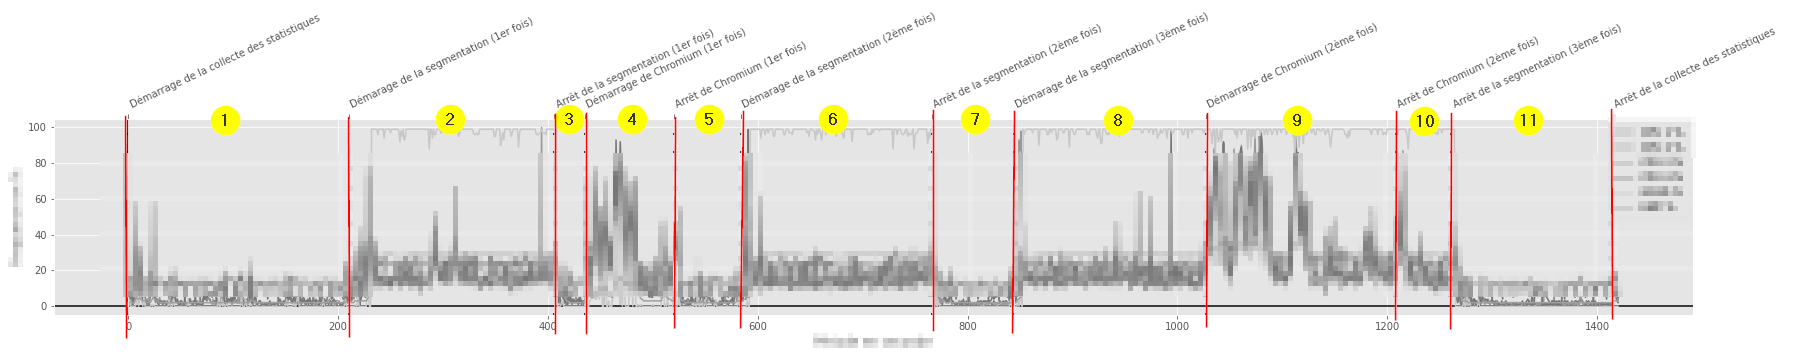
\includegraphics[width=1.0\textwidth]{test_periods}
   \caption{Les périodes du test}
   \label{fig:test_periods}
\end{figure}
{
   \clearpage 
   \newpage
   \begin{landscape}
   \begin{figure}[H]
      \centering
      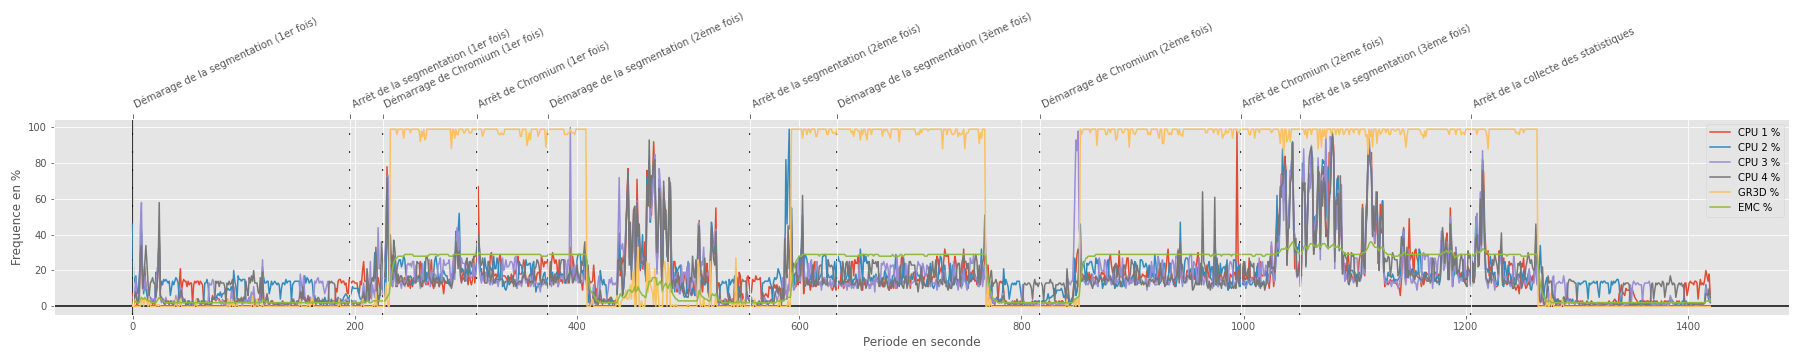
\includegraphics[width=1.5\textwidth]{frequency_usage}
      \caption{Fréquence}
      \label{fig:frequency_usage}
   \end{figure}
   \begin{figure}[H]
      \centering
      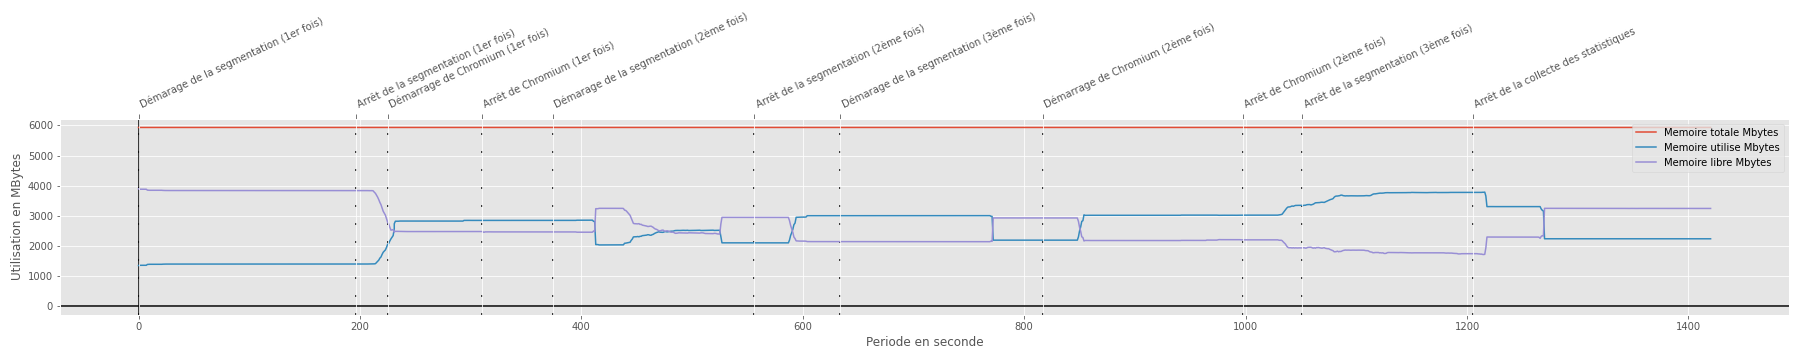
\includegraphics[width=1.5\textwidth]{memory_usage}
      \caption{Mémoire}
      \label{fig:memory_usage}
   \end{figure} 
   \begin{figure}[H]
      \centering
      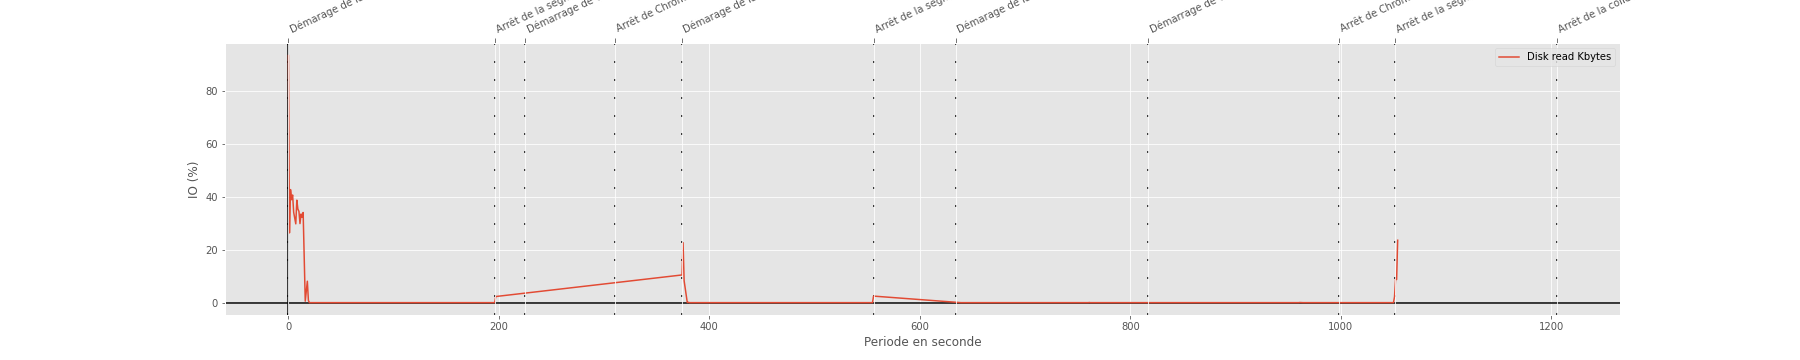
\includegraphics[width=1.5\textwidth]{io}
      \caption{I/O total en \% de la segmentation}
      \label{fig:io}
   \end{figure}
   \begin{figure}[H]
      \centering
      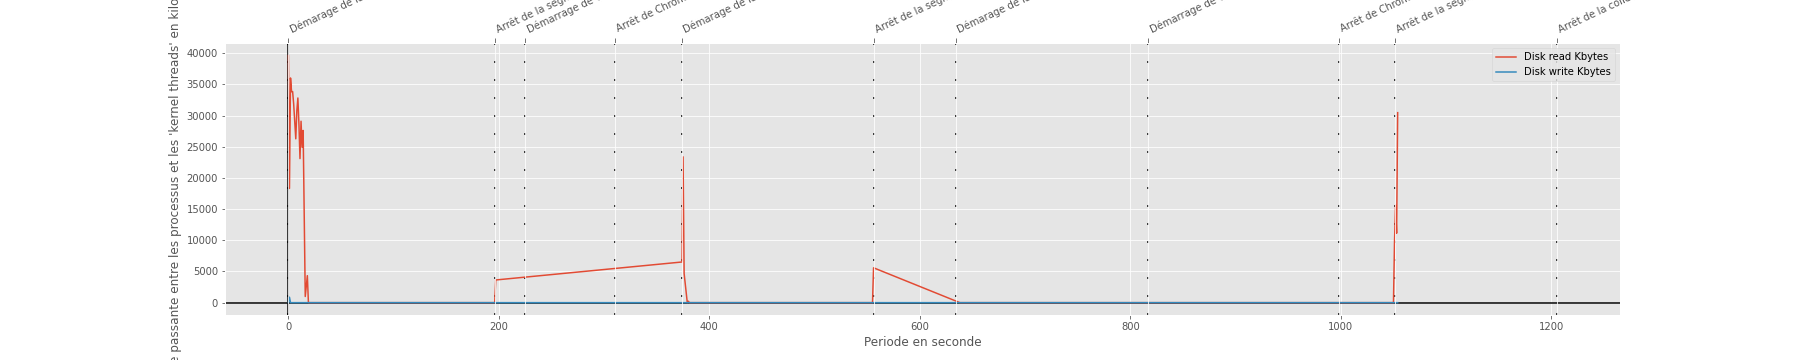
\includegraphics[width=1.5\textwidth]{io_segnetcamera}
      \caption{I/O en KBytes de la segmentation}
      \label{fig:io_segnetcamera}
   \end{figure} 
   \begin{figure}[H]
      \centering
      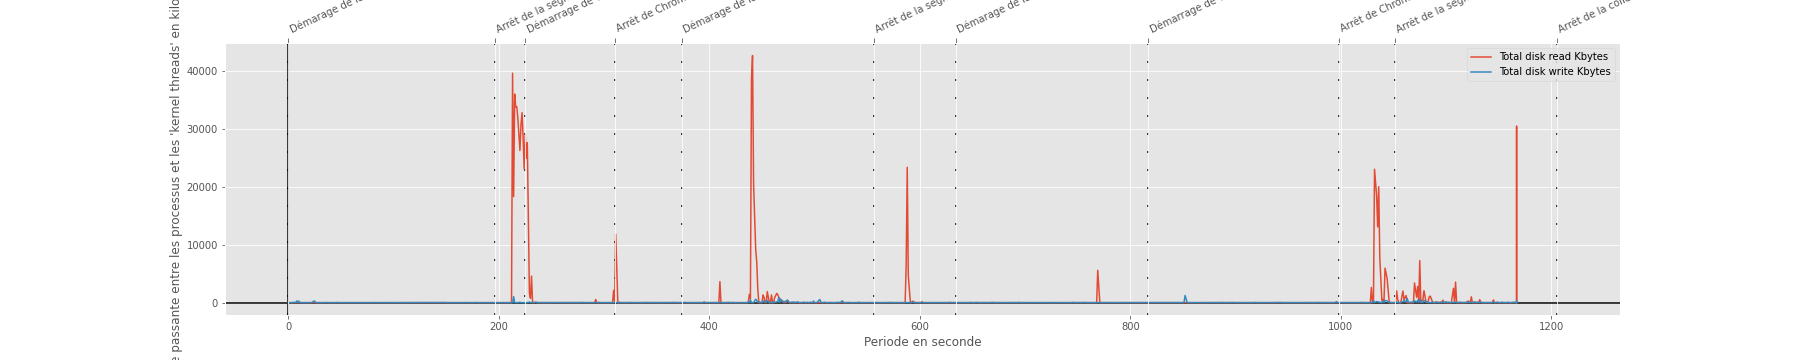
\includegraphics[width=1.5\textwidth]{io_totaldisk}
      \caption{I/O total du disque en KBytes}
      \label{fig:io_totaldisk}
   \end{figure} 
   \begin{figure}[H]
      \centering
      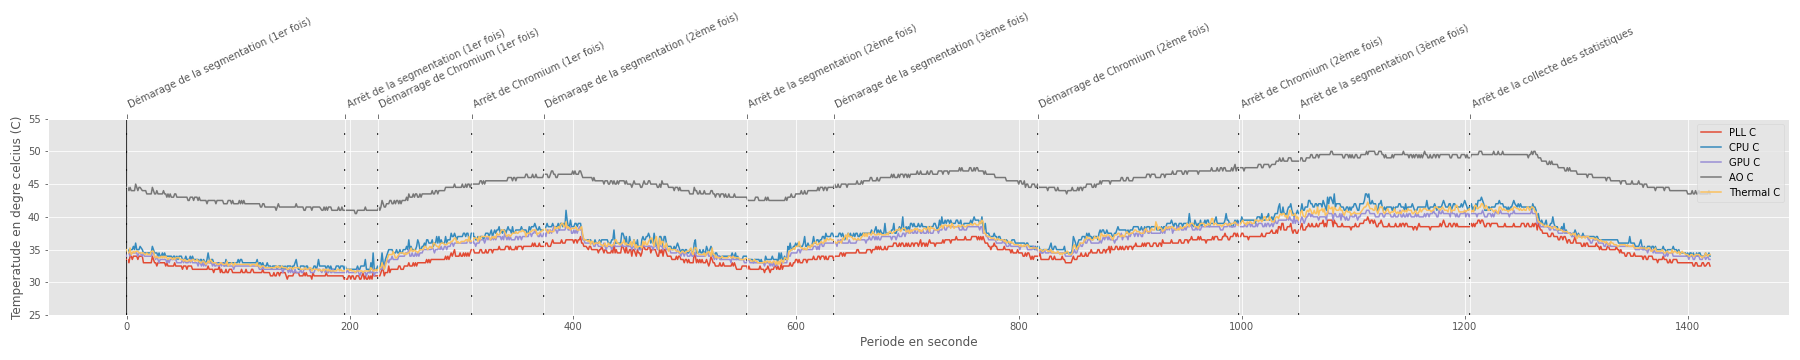
\includegraphics[width=1.5\textwidth]{temperature}
      \caption[Températures d'opération]{Températures d'opération\protect\footnotemark}
      \label{fig:temperature}
   \end{figure} 
   \footnotetext{PLL: Phase locking loop thermal sensor; AO: Always on thermal sensor. \url{https://forums.developer.nvidia.com/t/operating-temperature-range-on-jetson-nano/73555/10}}
   \begin{figure}[H]
      \centering
      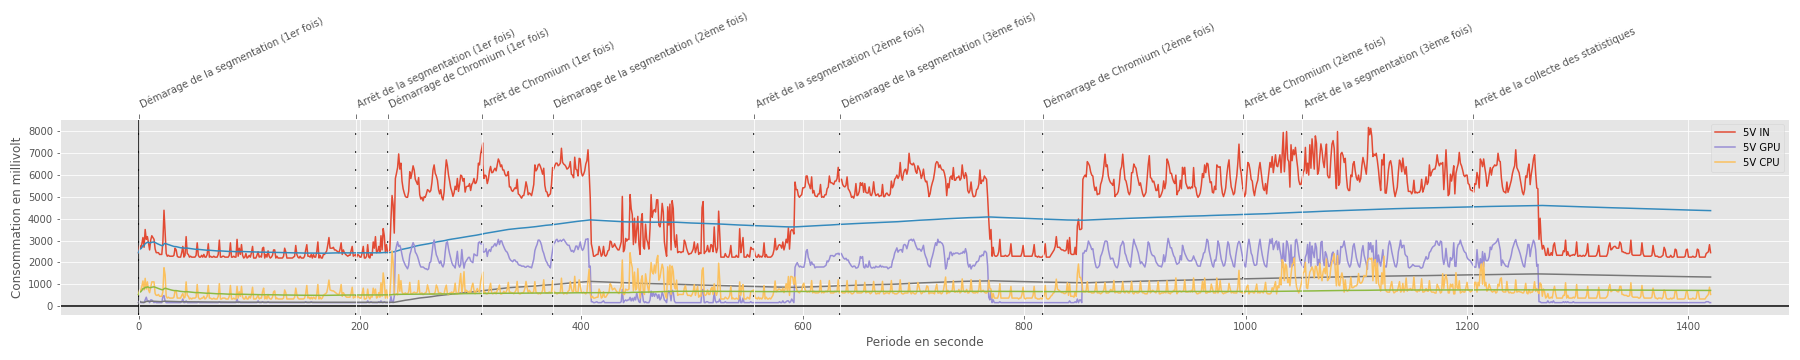
\includegraphics[width=1.5\textwidth]{consommation}
      \caption{Consommation d'opération}
      \label{fig:consommation}
   \end{figure}
   \end{landscape}
   \clearpage
   \newpage
}
\subsection{Performances de l'inférence}
\subsubsection{Images}
\par Les tests ont été faits avec le modèle "fcn-resnet18-deepscene-576x320" fourni par NVIDIA. 
\par Lors de l'entrainement et l'inférence, le script montre un \acrshort{iou} moyen du modèle de 75\%. Mais l'objet d'intérêt de l'essai n'est pas la qualité de la segmentation de l'image complète, mais seulement de la piste cyclable. Certains efforts ont dû être dépensés\footnote{\url{https://github.com/vince7lf/vince7lf.github.io/blob/master/_notebooks/2020-06-21-image_pred_color.ipynb}} afin de pouvoir observer le \acrshort{iou} et le "F1 score" de la segmentation sémantique de la piste cyclable uniquement.
\par Le résultat de la segmentation sémantique peut-être visualisé avec ces deux photos, prises du jeu de donnée de test de la forêt de Freiburg et utiliser comme jeu de données de test pour le modèle. L'image utilisée possède une version vérité terrain (\acrshort{gt}). L'image générée est l'image prédite et peut être comparée avec l'image vérité terrain (\acrshort{gt}), tant que la palette de couleur est identique à la version vérité terrain (\acrshort{gt}). 
\par Il s'avère que le \acrshort{iou} et "F1 score" sont assez élevés pour les deux photos. 
\par{
   \definecolor{trail}{RGB}{170, 170, 170}
   \definecolor{grass}{RGB}{0, 255, 0}
   \definecolor{vegetation}{RGB}{102, 102, 51}
   \definecolor{sky}{RGB}{0, 120, 255}
   \definecolor{obstacle}{RGB}{0, 0, 0}
   \tikz \fill [trail] (0.05, 0.05) rectangle (1.0, 0.5) ; {Chemin}
   \tikz \fill [grass] (0.05, 0.05) rectangle (1.0, 0.5) ; {Herbe}
   \tikz \fill [vegetation] (0.05, 0.05) rectangle (1.0, 0.5) ; {Végétation/arbres}
   \tikz \fill [sky] (0.05, 0.05) rectangle (1.0, 0.5) ; {Ciel}
   % \tikz \fill [obstacle] (0.05, 0.05) rectangle (1.0, 0.5) ; {Obstacle}
}
\par {\color{red}Ajout de la photo originale \todo{TODO}}
\begin{figure}[H]
   \centering
   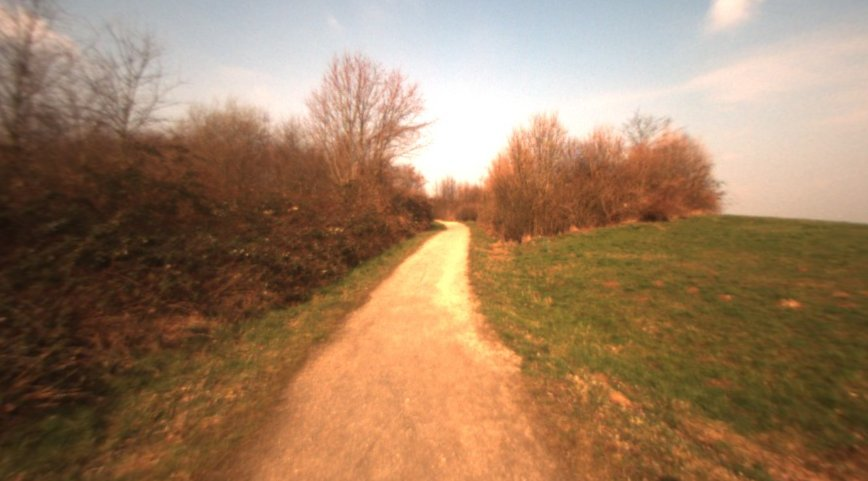
\includegraphics[width=0.75\textwidth]{b1-09517_Clipped}
   \caption{vérité terrain (\acrshort{gt}) de l'image b1-09517}
   \label{fig:b1-09517_Clipped}
\end{figure}
\begin{figure}[H]
   \centering
   
\includegraphics[width=0.75\textwidth]{b1-09517_Clipped_pred_new_color}
   \caption{Segmentation sémantique de l'image b1-09517 générée par le modèle. Le \acrshort{iou} et le "F1 score" pour le chemin sont de +80\%.}
   \label{fig:b1-09517_Clipped_pred_new_color}
\end{figure}
\par {\color{red}Ajout de la photo originale \todo{TODO}}
\begin{figure}[H]
   \centering
   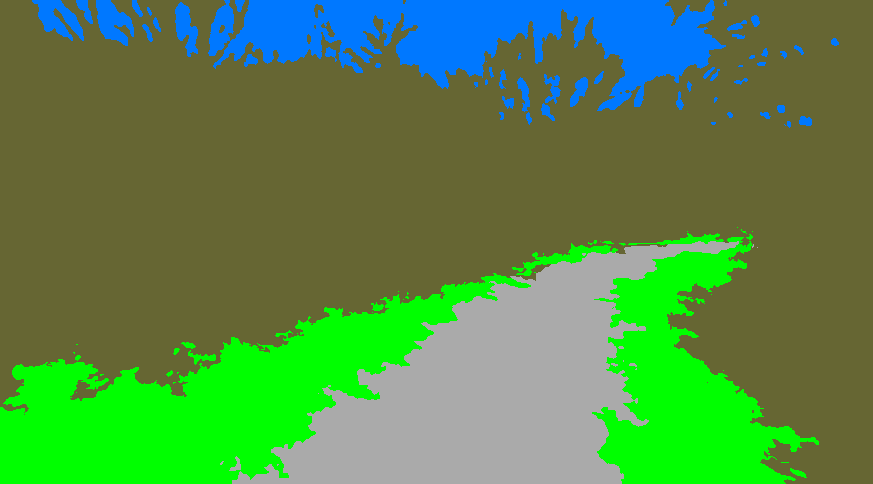
\includegraphics[width=0.75\textwidth]{b378-61_mask}
   \caption{vérité terrain (\acrshort{gt}) de l'image b378-61}
   \label{fig:b378-61_mask}
\end{figure}
\begin{figure}[H]
   \centering
   
\includegraphics[width=0.75\textwidth]{b378-61_mask_pred_new_color}
   \caption{Segmentation sémantique de l'image b378-61 générée par le modèle. Le \acrshort{iou} pour le chemin est +69\%.}
   \label{fig:b378-61_mask_pred_new_color}
\end{figure}
\subsubsection{Vidéos}
\par Il y a deux vidéos qui ont été utilisées pour tester les performances de la segmentation avec une vidéo. Comme il n'est pas évident de montrer une vidéo dans un essai, des liens sont mis à disposition. Ces vidéos sont disponibles dans le projet "Vision Météo" de Teams de l'université de Sherbrooke. Chaque vidéo a été créée en filmant avec un téléphone intelligent l'écran du nano ordinateur pendant que la segmentation est exécutée. Cela produit une vidéo HD 1080p 30 \acrshort{fps}. Lors de la seconde vidéo, les performances du système et les statistiques "tegrastats" sont affichées en plus de la segmentation.
\par J'ai tenté de capturer le résultat (vidéos/images) de l'inférence directement depuis le nano ordinateur, mais ce n'est pas une bonne idée, car trop intrusif, l'inférence est ralentie. Deux images sont produites par le modèle: "overlay" et "mask", qui sont directement rafraichies dans un XWindow. 
\begin{itemize}
   \item Lien\footnote{\url{https://usherbrooke.sharepoint.com/sites/ProjetVisionMto/Documents\%20partages/General/projet_visionmeteo/videos/gae724_lefv2603/resultats/20200221_020044.mp4}} vers une courte vidéo de 30 secondes démontrant l'inférence en temps réel de la segmentation sémantique d'une vidéo de la piste cyclable du pont Jacques-Cartier dans des conditions ensoleillée, mais avec un angle de vue qui change rapidement. Inférence effectuée en 30 \acrshort{fps} 1280x720 avec le modèle "fcn-resnet18-deepscene-576x320";
   \item Lien\footnote{\url{https://usherbrooke.sharepoint.com/sites/ProjetVisionMto/Documents\%20partages/General/projet_visionmeteo/videos/gae724_lefv2603/resultats/20200412_232155.mp4}} vers une vidéo longue de +8 minutes présentant l'inférence en temps réel de la segmentation sémantique d'une vidéo d'une piste cyclable dans des conditions ensoleillée, mais mouillée, avec présence de neige. Durée de plus de 8 minutes. La taille de la vidéo est de 800Mb. La même vidéo, d'une durée de 30 secondes, est utilisée successivement avec différentes images par seconde (60 / 30 / 15 / 1 \acrshort{fps}) et résolutions (720x1280 / 480x640 / 320x480 / 240x320). Le modèle est "fcn-resnet18-deepscene-576x320". Selon le titre de la fenêtre xWindow présentant la segmentation, le \acrshort{fps} est autour de 23-26 \acrshort{fps}.
\end{itemize}
\par Voici un tableau montrant les différentes résolutions et images par seconde (\acrshort{fps}) qui ont été testées avec le modèle:
{
    \renewcommand*{\arraystretch}{1.4}
    \begin{table}[ht]
    \centering
    \caption{Résolutions et images par seconde (\acrshort{fps}) testés}\label{table:resolutions_tested}
    \vspace{0.1em} % Adjust the height of the space between caption and tabular
    \begin{tabular}{{@{}|p{12cm}|@{}}}
         \hline
         \textbf{Résolutions qui fonctionnent}\\
         \hline
        320x576, 480x640, 720x1280, 768x1024, 768x1152, 800x1152, 832x1024, 864x1024\\
        \hline
        \textbf{Résolutions qui ne fonctionnent pas}\\
        \hline
        832x1120, 832x1152, 768x1280, 800x1280, 864x1152, 900x1152, 900x1280, 960x1600, 1080x1920, 1024x1024\\
        \hline
        \textbf{Images par seconde (\acrshort{fps}) supportées}\\
        \hline
        60/1, 30/1, 15/1, 1/1\\
        \hline
    \end{tabular}
    \end{table}
}